\documentclass[../manuscript.tex]{subfiles}
\section{Введение}
\subsection{Основные концепции Хемоинформатики}

Хемоинформатика, согласно определению данному Й. Гастайгером \cite{gasteiger2006chemoinformatics}, - это применение методов информатики для решения химических задач. Одна из основополагающих задач в химии это создание соединений с заданными свойствами. Моделирование (количественных) соотношений "структура-активность" ((Q)SAR, Quantitative Structure-Activity Relationships) позволяет выявить взаимосвязь между структурой химических соединений и их активностью, чаще всего биологической. Модели SAR широко используются для виртуального скрининга при разработке лекарств с целью сокращения количества экспериментальных испытаний. Становление химии как науки привело к накоплению огромного количества данных, поэтому возникла необходимость ими оперировать: хранить информацию о миллионах химических соединениях и осуществлять быстрый поиск в этой информации. Более того, количество потенциальных химических соединений почти бесконечно, например, существует более $10^{29}$ возможных производных н-гексана со 150 заместителями \cite{lipinski2004navigating}. Для работы с такими объемами информации требовалось создать машиночитаемое представление химических структур. Оно должно быть уникальным и однозначно интерпретируемым. 
% Я подредактировала введение, так как ты пишешь про две основные задачи в хемоинформатике и их надо разбить - организацию хранения и поиска информации и построение моделей структура-активност.

\subsubsection{Представление}
Представление структур химических соединений делится на 2 типа:
\begin{itemize}
    \item внутреннее
    \item внешнее
\end{itemize}

$$\textbf{Внутреннее представление}$$


Когда говорят о внутреннем представлении структур химических соединений подразумевается машинное представление. Для внутреннего представления обычно используются молекулярные графы. Молекулярный граф — связный граф, находящийся во взаимно-однозначном соответствии со структурной формулой химического соединения таким образом, что вершинам графа соответствуют атомы молекулы, а ребрам графа — химические связи между этими атомами. Такое представление не хранит информацию о трехмерной структуре молекулы. Обычно граф неориентированный (связи в молекуле не имеют направления) и его вершины помечены (символами атомов) \cite{gasteiger2006chemoinformatics}. Если вершины графа непомечены, то он будет отражать только структуру, а не состав молекулы. Две вершины графа могут соединяться несколькими ребрами, так как связь может быть одинарной или кратной.


Граф может быть представлен в виде матрицы разными способами, например матрицей смежности, расстояний, инцидентности.


Матрица смежности для молекулы, состоящей из n атомов, это квадратная матрица размером $n\times{n}$, содержащая информацию о всех связях в молекуле. Если на пересечении i-ой строки и j-ого столбца стоит 1, то между соответствующими атомами есть связь. Если нет связи между рассматриваемыми атомами, то на соответствующей позиции матрицы стоит 0. То есть матрица смежности является Булевой матрицей. Все диагональные элементы матрицы равны 0 и она является симметричной. Такая матрица является избыточной. Ее можно упростить, устранив	дублирование половины матрицы, то есть приведя к верхней треугольной матрице. Также для ясности можно упустить нули и удалить	информацию	об	атомах	водорода \cite{gasteiger2006chemoinformatics}.

\begin{figure}[H]
\center{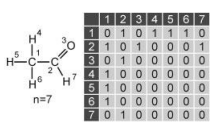
\includegraphics[width=0.5\linewidth]{images/матрица смежности с молекулой.png}}
\caption{Матрица смежности этанола \cite{gasteiger2006chemoinformatics}}
\end{figure}

\begin{figure}[h!]
\center{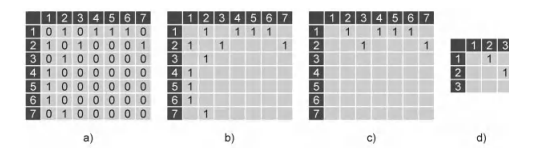
\includegraphics[width=0.9\linewidth]{images/разные матрицы смежности.png}}
\caption{a) избыточная матрица смежности этанола; b)матрица после опускания нулей; c) упрощенная до верхней треугольной матрицы; d) после удаления атомов водорода \cite{gasteiger2006chemoinformatics}}
\end{figure}


Для примера рассмотрим матрицу расстояний, у которой ее элемент представляет кратчайшее расстояние между соответствующими атомами. Расстояние может выражаться в геометрическом расстоянии (ангстремах) или топологическом расстоянии (числе связей) \cite{gasteiger2006chemoinformatics}.

\begin{figure}[H]
\center{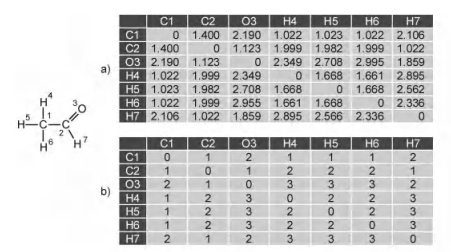
\includegraphics[width=0.7\linewidth]{images/матрица расстояний.png}}
\caption{матрица расстояний этанола с a) геометрическим расстоянием; b) топологическим расстоянием \cite{gasteiger2006chemoinformatics}}
\end{figure}


Еще одним представлением является матрица инцидентности. Это матрица размером $n\times{m}$, где n-число вершин(атомов), m - число ребер (связей). Если на пересечении i-ой строки и j-ого столбца стоит значение 1, то рассматриваемые вершина и ребро инцидентные \cite{gasteiger2006chemoinformatics}.

\begin{figure}[h!]
\center{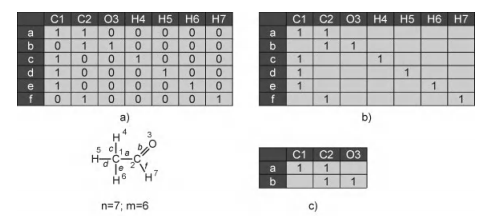
\includegraphics[width=0.9\linewidth]{images/матрица инд.png}}
\caption{a) избыточная матрица инцидентности этанола; b) матрица после опускания нулей; c) после опускания атомов водорода \cite{gasteiger2006chemoinformatics}}
\end{figure}

Все описанные матрицы не несут информации о типе и  порядке связей в молекуле.

Одним из недостатков матрицы смежности является, что число ее элементов равно квадрату числа атомов, а для представления молекулярного графа необходимо, чтобы число элементов в представлении линейно зависело от числа атомов в молекуле. Это достигается с помощью представления таблицей связности, в которой дается список атомов и список связей. Существует много вариантов матриц связности. Например, атомы произвольно нумеруются и в соответствии с индексом заносятся в список атомов. Информация о связях хранится во второй таблице, где для каждой связи записываются индексы атомов, которые она соединяет и ее кратность \cite{gasteiger2006chemoinformatics}.

\begin{figure}[H]
\center{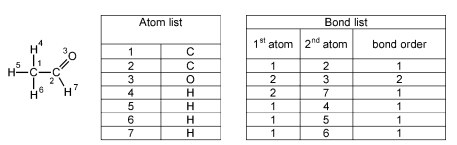
\includegraphics[width=0.9\linewidth]{images/таблица связанности.png}}
\caption{таблица связности этанола}
\end{figure}

Другой формой представления является таблица, в которой первые две колонки содержат информацию о индексах и символах атомов. Далее таблица дополняется колонками, в которых указаны индексы соседних атомов и кратность связи. Такая форма представления избыточна, в ней каждая связь записана дважды. Ее можно упростить, убрав повторение связей и опустив атомы водорода.
\begin{figure}[H]
\center{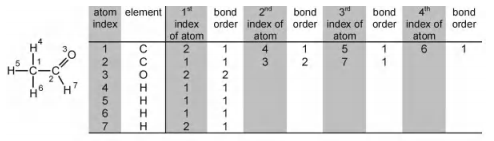
\includegraphics[width=0.9\linewidth]{images/вторая форма таблицы связанности.png}}
\caption{таблица связности этанола \cite{gasteiger2006chemoinformatics}}
\end{figure}
 
Таблицы связности могут быть дополнены другими списками, например содержащими информацию о свободных электронах или заряде атомов, что является еще одним преимуществом по сравнению с матрицами смежности \cite{gasteiger2006chemoinformatics}.

Методы теории графов находят широкое применение в хемоинформатике. 
$$\textbf{Внешнее представление}$$


Внешнее представление химических соединений используется в случае долговременного хранения химической информации и обмена ею между приложениями.


Простейшим типом внешнего представления структур химических соединений являются линейные нотации в виде строки символов.
Линейные нотации позволяют свободно обмениваться информацией о химических соединениях без необходимости использования специального программного обеспечения. Наиболее популярные типы линейных нотаций:

\begin{itemize}
\item SMILES (Simplified Molecular Input Line Entry System);
\item SMARTS (расширение SMILES )
\item InChI (IUPAC International Chemical Identifier)
\end{itemize}

В настоящее время наиболее распространённым видом линейных нотаций являются строки SMILES. Преобразование структуры соединения в строку символов SMILES определяется 6 правилами \cite{gasteiger2006chemoinformatics} :
\begin{itemize}
\item Атомы представлены их атомными символами.
\item Атомы водорода опущены
\item Соседние атомы расположены рядом друг с
другом.
\item Двойные и тройные связи характеризуются «=» и
«#», соответственно.
\item Разветвления молекулы представлены скобках.
\item Циклы описаны путем выделения цифры для двух "соединяющихся" атомов в цикле. 
\end{itemize}

Синтаксис SMILES позволяет описывать структурные изомеры. SMARTS является расширением SMILES для поисковых запросов в химических базах данных. 

Для кодировки химических структур IUPAC предложил универсальную линейную нотацию InChI. То есть это цифровой эквивалент названию соединения по номенклатуре IUPAC. Он содержит следующие уровни информации: связанность, таутомеризм, изотопы, стереохимия, заряд. Этот формат более сложен для интерпретации пользователем, но сохраняет такую возможность.

InChIKey – хешированная версия InChI, созданная для
быстрого поиска.

Второй тип внешнего представления структур химических соединений основан на непосредственном кодировании таблицы связности молекулярного графа. Такие распространённые форматы как MOL, SDF и RDF, которые в настоящее время являются стандартными для обмена химической информацией, можно считать способами представления в виде текстового файла матрицы смежности молекулярного графа.

\subsubsection{Молекулярные дескрипторы}

Традиционный подход к обработке химической информации состоит в отображении химического пространства на дескрипторное пространство, образуемое вычисляемыми для каждого химического объекта векторами молекулярных дескрипторов — числовых характеристик, описывающих химические объекты. Это дает возможность применять методы математической статистики и машинного обучения для работы с химическими объектами.  В  принципе дескриптором может являться любое число, которое можно рассчитать из структурной формулы химического соединения. Молекулярные дескрипторы можно классифицировать по "размерности": 0D , 1D, 2D, 3D и 4D. 0D дескрипторы описывают совокупную информацию, такую как количество атомов, количество связей, молекулярный вес. 1D дескрипторы описывают число фрагментов в молекуле. В качестве примера можно привести число гидроксильных групп, нитрогрупп \cite{gasteiger2006chemoinformatics}. 2D дескрипторы описывают свойства, которые могут быть вычислены из
двумерного представления молекул (например, индексы связности) и 3D-дескрипторы зависят от конформации молекул (например,
доступная растворителю площадь поверхности) \cite{xue2000molecular}.
 
\subsubsection{Молекулярные отпечатки}
Молекулярные «отпечатки» (molecular fingerprints) содержат информацию о присутствии или
отсутствии определенных признаков в химическом соединении, например, фрагментов.
Могут	быть	организованы	2	основными	способами:
\begin{itemize}
    \item бинарной строки
    \item хеш-таблицы
\end{itemize}

Рассмотрим подробнее молекулярные отпечатки в виде бинарной строки. Каждая подструктура или фрагмент активирует определенное количеств позиций (битов) в молекулярном отпечатке. Иногда подструктуре может соответствовать 1 или несколько битов. Алгоритм определяет какие биты были активированы подструктурой. Одна и та же подструктура всегда активизирует одинаковые биты. Если фрагменту соответствует 1 бит, то в случае равенства единице, то фрагмент присутствует в молекуле, иначе его значение равно нулю. Обычно длина бинарной строки 150-2500 битов. Алгоритм работает таким образом,
что всегда возможно ассоциировать биты с конкретной подструктурой. Однозначное представление химической структуры строкой позволяет проводить эффективный поиск схожих молекул. 

Для хэшированных молекулярных отпечатков нет возможности определить, какие конкретные элементы присутствуют в молекуле.



\subsubsection{Молекулярное подобие}

В основе принципа молекулярного подобия лежит идея, что структурно схожие молекулы предположительно обладают сходной биологической активностью. Однако это предположение не всегда может быть верным. Например, "activity cliffs", в которых незначительная модификация функциональных групп вызывает резкое изменение активности \cite{lo2018machine}. Поиск структурного сходства молекул основан на доле различных фрагментов, которые присутствуют одновременно в обеих молекулах. Поиск молекул по такому критерию называется поиском по молекулярному подобию (Similarity Search). В качестве количественной меры молекулярного подобия часто рассматривается величина, возрастающая с уменьшением расстояния между химическими соединениями в дескрипторном пространстве.

Структурное сходство двух молекул чаще всего оценивается путем вычисления коэффициента Танимото (Tc). Tc, также известный как индекс Джаккарда, описывает степень схожести двух множеств. Для  парного сравнения используются молекулярные отпечатки молекул. Коэффициент Танимото определяется как :

\begin{equation}
    Tc=\frac{bc}{b1+b2-bc},
    \label{equation1}
\end{equation}
где b1 - число битов набора первой молекулы, b2 - число битов набора второй молекулы, bc - число битов общих для обеих молекул. Значения коэффициента Танимото лежит в пределах от 0 до 1 \cite{xue2000molecular}. Высокие значения Тc
указывают на то, что два соединения похожи, но не дает информации о масштабах сходства, например о том, какие конкретные химические группы они разделяют.

\subsection{Синергия}
Под комбинированной терапией подразумевают одновременное применение нескольких препаратов.

Существует три типа эффектов от комбинации препаратов: 
\begin{itemize}
    \item аддитивный, когда комбинированный эффект эквивалентен сумме независимых эффектов
    \item синергический, когда комбинированный эффект больше аддитивного
    \item антагонистический, когда комбинированный эффект меньше аддитивного
\end{itemize}

Целью комбинированной терапии является достижение синергического или, по крайней мере, аддитивного, но комплементарного эффекта \cite{bansal2014community, li2018network}

\subsubsection{Область применения синергии}
Большинство заболеваний вызвано сложными биологическими процессами. Широко известным примером являются онкологические заболевания. На данный момент разработана таргетная терапия рака, которая блокирует рост раковых клеток с помощью вмешательства в механизм действия конкретных целевых (таргетных) молекул, необходимых для канцерогенеза, то есть ингибирует критические сигнальные пути рака. Как и ожидается, такая терапия будет более эффективной, чем прежние виды лечения, и менее вредной для нормальных клеток. Однако за резким начальным положительным ответом многих таргетных методов лечения рака часто следует развитие лекарственной устойчивости, приводящей к рецидиву заболевания\cite{huang2019driver}. Существует множество механизмов, которые могут привести к лекарственной устойчивости, которые включают генетическую и негенетическую гетерогенность, присущую распространенным видам рака, в сочетании со сложными механизмами обратной связи и регуляции, а также динамическими взаимодействиями между опухолевыми клетками и их микроокружением. Любая
монотерапия может быть ограничена по своей эффективности, но комбинации лекарств потенциально могут преодолеть эти ограничения \cite{kuiper2019community}. Они состоят из нескольких агентов, каждый из которых обычно используется в клинике как один эффективный препарат. Поскольку агенты в лекарственных комбинациях могут модулировать активность отдельных белков, лекарственные комбинации могут помочь повысить терапевтическую эффективность, преодолев избыточность, лежащую в основе лекарственной устойчивости. Соответственно приводят к более длительным реакциям у пациентов\cite{zhao2011prediction}.

Кроме того, токсичность и неблагоприятные побочные эффекты, вероятно, снижаются, поскольку дозы комбинаций лекарств обычно ниже, чем дозы отдельных агентов. В настоящее время медикаментозная комбинаторная терапия становится перспективной стратегией лечения многофакторных сложных заболеваний \cite{preuer2018deepsynergy}.

Также необходимо упомянуть еще одну возможную область применения синергии - химическое перепрограммирование клеток малыми молекулами. Точнее, эта область нуждается в использовании комбинаций малых молекул, так как при переходе из одного клеточного состояния в другое происходят большие изменения в фенотипе и обработки клетки одним соединением недостаточно. 

\subsubsection{Предсказание синергетических пар соединений}

Изначально эффективные комбинации препаратов предлагались на основе клинического опыта и большинство подходов к выявлению синергетических пар соединений часто носит экспериментальнй характер. В исследованиях рака анализ синергизма обычно проводится путем обработки клеточных линий \emph{in vitro} всеми возможными комбинациями соединений. Однако такой подход требует много усилий и затрат. Более того, экспериментальные скрининги накладывают серьезные ограничения на практический размер библиотек и их разнообразие. Вычислительные методы прогнозирования синергии соединений потенциально могут позволить исследователям отбирать наиболее перспективные пары для экспериментального скрининга, и, вследствие сокращения количества изучаемых комбинаций, сократить затраты ресурсов \cite{bansal2014community}.

Большинство существующих методов скрининга нацелены на прогнозирование синергических эффектов двух препаратов, поскольку комбинаторный эффект трех и более препаратов технически сложнее предсказать и практически отсутствуют экспериментальные данные для последующей валидации метода\cite{li2018network}. Также есть наблюдения, что наиболее значительное улучшение достигается при добавлении только одного дополнительного препарата. При дальнейшем добавления лекарств эффективность постепенно уменьшается и в конечном счете достигает плато \cite{napolitano2020automatic}.


На молекулярном уровне синергетические взаимодействия могут быть реализованы несколькими различными механизмами. Например, соединение может сенсибилизировать клетки к другому соединению, регулируя его поглощение и распределение, моделируя ростовые свойства клетки, ингибируя деградацию соединения, ингибируя пути, индуцирующие резистентность или снижая токсичность другого соединения \cite{bansal2014community}.

Механизмы синергических эффектов не являются универсальными среди различных лекарств или раковых заболеваний \cite{li2018network}.

Можно выделить две гипотезы, лежащие в предсказании синергии препаратов \cite{bansal2014community}:
\begin{itemize}
    \item гипотеза сходства: соединения, более схожие по вызываемым транскрипционным изменениям, с большей вероятностью будут синергетическими
    \item гипотеза комплиментарности: соединения, которые вызывают наиболее различные, но взаимодополняющие транскрипционные изменения, с большей вероятностью будут синергетическими (так как мы ищем синергетические пары среди препаратов с определенным необходимым эффектом, то можно сказать, что по гипотезе несходства синергетические соединения комплементарно дополняют друг друга в достижении желаемого эффекта)
\end{itemize}



На данный момент отсутствуют стандартные подходы к прогнозированию активности пар соединений на основе транскриптомных данных \cite{bansal2014community}.

Поиск синергетических пар можно представить в виде задачи регрессии, когда необходимо предсказать уровень синергии пары препаратов. Эта же задача может быть представлена в виде ранжирования списка пар препаратов по степени синергии \cite{bansal2014community}. Но также можно рассматривать более простую задачу бинарной классификации, когда необходимо сказать, является пара препаратов синергетической или нет \cite{kuiper2019community}.

Данные, используемые для предсказания синергии, можно поделить на несколько типов:
\begin{itemize}
    \item глубокая молекулярная характеристика клеточных линий, которая включает  соматические мутации, изменения числа копий, метилирование ДНК и профили экспрессии генов 
    \item фармокологические признаки препаратов, включая предполагаемые лекарственные мишени и химические свойства препаратов, представленные дескрипторами и молекулярными отпечатками, области медицинских показаний, побочные эффекты и токсикофоры, сигнальные пути
    \item данные монотерапии, включающие зависимость жизнеспособности клеток от дозы препарата при обработке одиночным препаратом, транскрипционные данные (профиль экспрессии генов клеток после обработки препаратом)
\end{itemize}

Безусловно, признаки типа клеточной линии существенны, так как они определяют молекулярный контекст. \cite{kuiper2019community}. Признак "сигнальный путь" слабо предсказательный, возможно, потому, что простая ассоциация между лекарствами и путями через целевые белки недостаточно отражает физиологический контекст, в котором работают лекарства \cite{zhao2011prediction}. Также плохой плохой предсказательной способностью обладает признак "побочные эффекты", потому что он сильно зашумлен, так как существуют некоторые общие побочные эффекты, связанные с большинством лекарств. Эффективность признака побочных эффектов может быть улучшена, если рассмотреть только тяжелые побочные эффекты, связанные с лекарствами \cite{zhao2011prediction}. Монотерапия дает существенную информацию о прямом лечебном эффекте на линию раковых клеток, что является основой лекарственного синергизма. Например, если препарат вообще не действует на определенную клеточную линию, он вряд ли будет синергировать с другими препаратами \cite{li2018network}. Однако такой признак, как зависимость жизнеспособности клеток от дозы препарата, в основном используется для поиска пар противопухолевых препаратов и не подходит для химического перепрограммирования. Также наблюдалась информативность транскрипционных данных, поскольку профили геномной экспрессии очень динамичны и зависят от контекста \cite{sun2015combining}.

Однако различные типы данных дополняют друг друга при прогнозировании комбинаций лекарственных средств \cite{zhao2011prediction}. То есть использование ансамбля различных наборов признаков улучшает качество  прогноза \cite{kuiper2019community}.

Кроме того, по предоставленному набору данных задачу поиска синергетических пар можно реализовывать в двух сценариях \cite{ding2019incorporating}:
\begin{itemize}
    \item  для предсказания уровня синергии пар препаратов предоставляются только данные по используемым клеточным линиям, фармакологические признаки препаратов, данные монотерапии 
    \item  для предсказания уровня синергии пар препаратов помимо вышеперечисленных данных предоставляется обучающий набор данных, который, например, может состоять из других пар препаратов, для которых будут доступны данные по клеточным линиям, фармакологические признаки препаратов, данные монотерапии и также известно, какие пары препаратов являются синергетическими, какие нет. В данном случае возможно применять методы машинного обучения.
\end{itemize}

В реальности предоставляемые данные бывают очень разнообразными, поэтому может применяться и смешанный сценарий, то есть использовать обучение с частичным привлечением учителя \cite{sun2015combining}.

Если в работе используется сценарий обучения с учителем, то либо известны синергетические комбинации, либо есть экспериментальные данные жизнеспособности клеток после обработки комбинациями препаратов в зависимости от дозы, по которым рассчитывается синергетический эффект.

Среди подходов к моделированию лекарственной синергии популярны методы машинного обучения. Однако труднодоступность обучающих данных препятствует широкому использованию методов машинного обучения. Используются следующие подходы: регрессия, деревья решений, случайные леса, Гауссовские процессы, SVM, нейронные сети. При сравнении моделей был сделан вывод, что класс алгоритмов показал слабую связь с производительностью метода \cite{kuiper2019community}.

Так как предсказание синергии можно отнести к задаче бинарной классификации, то популярны метрики ROC-AUC, accuracy, precision, recall, F1 \cite{zhao2011prediction, sun2015combining}. Рассмотрим их подробнее.
Наши данные поделены на два класса. Их метки принято обозначать как «положительные»  и «отрицательные». При классификации мы можем верно определить класс (истинно) или допустить ошибку, то есть отнести к ложному классу, поэтому возможны следующие исходы: 
\begin{itemize}
    \item истинно положительные (TP)
    \item истинно отрицательные (TN)
    \item ложно положительные (FP)
    \item ложно отрицательные (FN)
\end{itemize}
\begin{figure}[H]
\center{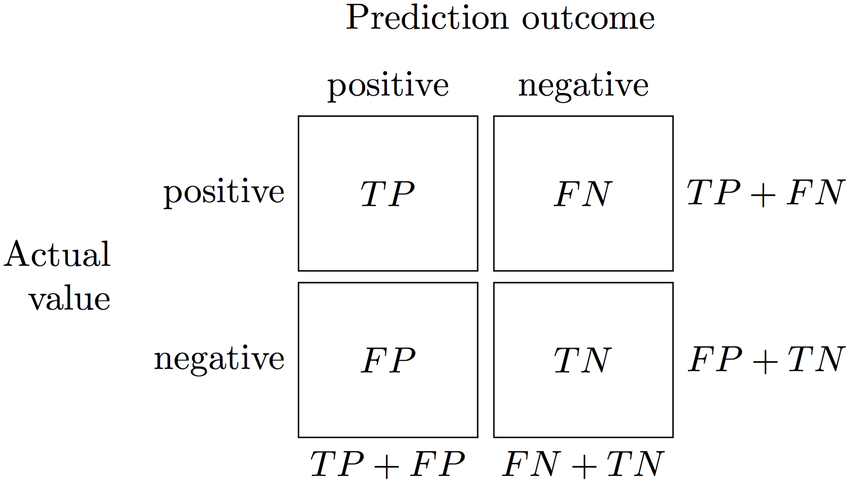
\includegraphics[width=0.5\linewidth]{images/confusion_matrix.png}}
\caption{Матрица сопряженности возможных результатов бинарной классификации}
\end{figure}

Одной из наиболее простых метрик является точность (accuracy). Она показывает количество верно классифицированных объектов (истинно положительных и истинно отрицательных) относительно общего количества всех объектов и считается следующим образом:
\begin{equation}
    accuracy = \frac{TP+TN}{TP+FP+TN+FN}
    \label{equation}
\end{equation}
Метрика accuracy имеет недостаток: она не подходит для несбалансированных классов, где может быть много экземпляров одного класса и мало другого.

Для оценки качества работы алгоритма на каждом из классов по отдельности вводятся метрики precision (точность) и recall (полнота).

Метрика precision показывает сколько из всех объектов, которые классифицируются как положительные, действительно являются положительными, относительно общего количества полученных от модели позитивных меток.
\begin{equation}
    precision = \frac{TP}{TP+FP}
    \label{equation}
\end{equation}
Важность этой метрики определяется тем, насколько высока для рассматриваемой задачи «цена» ложно положительного результата.

Метрика recall  показывает, сколько объектов модель смогла правильно классифицировать с позитивной меткой из всего множества позитивных. Она вычисляется по следующей формуле:
\begin{equation}
    recall = \frac{TP}{TP+FN}
    \label{equation}
\end{equation}
Необходимо уделить особое внимание этой оценке, когда в поставленной задаче ошибка не распознать положительный класс высока.

\begin{figure}[H]
\center{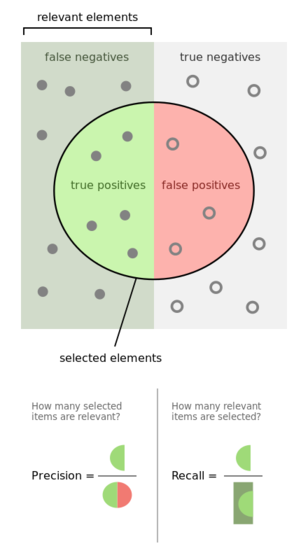
\includegraphics[width=0.3\linewidth]{images/precision-recal.png}}
\caption{Схематичное представление precision и recall}
\end{figure}
Precision и recall не зависят, в отличие от accuracy, от соотношения классов и потому применимы в условиях несбалансированных выборок. Если Precision и Recall являются одинаково значимыми, то можно использовать их среднее гармоническое для получения оценки результатов:

\begin{equation}
    F1-score = \frac{2\cdot{recall}\cdot{precision}}{recall+precision}
    \label{equation}
\end{equation}

Для определения бинарной метки (0 или 1) по какому-нибудь вещественному ответа алгоритма (как правило, вероятности принадлежности к классу) необходимо выбрать порог, до которого ставится метка "0", после "1". Порог, равный 0.5 кажется естественным, но он не всегда оказывается оптимальным, например, при отсутствии баланса классов.


Одним из способов оценить модель в целом, не привязываясь к конкретному порогу, является метрика ROC AUC — площадь (Area Under Curve) под кривой ошибок (Receiver Operating Characteristic curve ). Данная кривая представляет из себя линию от (0,0) до (1,1) в координатах True Positive Rate (TPR) и False Positive Rate (FPR).

True Positive Rate (Recall) показывает долю верно классифицируемых объектов положительного класса и считается по формуле:
\begin{equation}
    TPR = \frac{TP}{TP+FN}
    \label{equation}
\end{equation}
False Positive Rate показывает, какую долю из объектов отрицательного класса алгоритм предсказал неверно, и определяется как:
\begin{equation}
    FPR = \frac{FP}{FP+TN}
    \label{equation}
\end{equation}

Когда классификатор не делает ошибок (FPR = 0, TPR = 1) мы получим площадь под кривой, равную единице; в противном случае, когда классификатор случайно выдает вероятности классов, AUC-ROC будет стремиться к 0.5, так как классификатор будет выдавать одинаковое количество TP и FP.
Каждая точка на графике соответствует выбору некоторого порога. Площадь под кривой в данном случае показывает качество алгоритма (больше — лучше), кроме этого, важной является крутизна самой кривой — надо максимизировать TPR, минимизируя FPR, а значит, кривая в идеале должна стремиться к точке (0,1).
\begin{figure}[H]
\center{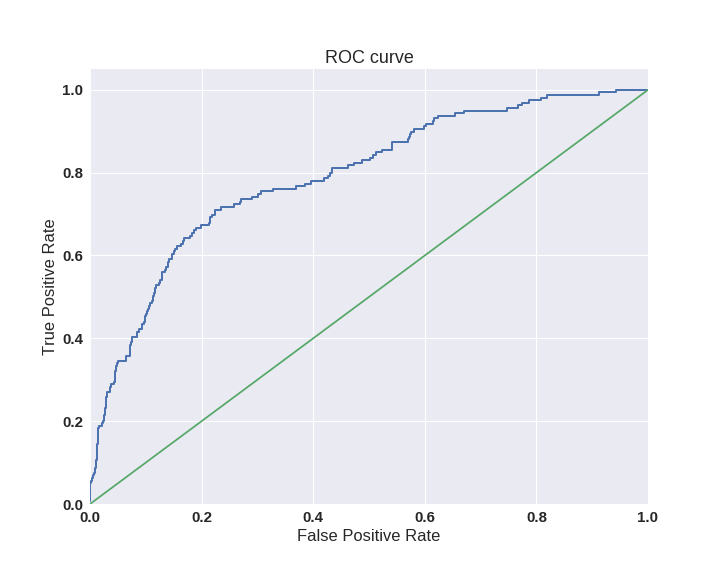
\includegraphics[width=0.7\linewidth]{images/ROC AUC.png}}
\caption{ROC кривая}
\end{figure}

Для задачи регрессии используется MSE, RMSE, коэффициент корреляции Пирсона \cite{preuer2018deepsynergy}.Рассмотрим их подробнее.


Метрика Mean Squared Error (MSE). Измеряет среднюю сумму квадратной разности между фактическим значением и прогнозируемым значением для всех объектов выборки. Возведение во вторую степень необходима, чтобы отрицательные значения не компенсировались положительными. Чем больше разность, тем больше ее вес в этой метрики. Ниже приведена ее формула.
\begin{equation}
    MSE = \frac{1}{n}\sum\limits_{i=1}^n{(y_i-{y_i}^{\text{pred}})^2}
    \label{equation}
\end{equation}


Метрика Root Mean Squared Error (RMSE) - это корень от квадрата ошибки. Формула приведена ниже.
\begin{equation}
    RMSE = \sqrt{\frac{1}{n}\sum\limits_{i=1}^n{(y_i-{y_i}^{\text{pred}})^2}}
    \label{equation}
\end{equation}

Также в соревновании консорциума DREAM использовалась PC-метрика, которая будет рассмотрена ниже \cite{bansal2014community}, \cite{kuiper2019community}, \cite{li2018network}, \cite{sun2015combining}.

Для проверки предсказанных синергетических пар используются экспериментальные данные и литература \cite{sun2015combining}.

Ниже описаны некоторые методы предсказания синергии, начиная с первого сценария, когда недоступен обучающий набор данных. В качестве примера необходимо упомянуть соревнования, проводимые консорциумом \href{http://dreamchallenges.org/}{DREAM Challenges}. 
\newline
\newline
\textbf{Методы предсказания синергии, разработанные на основе \\наборов данных консорциума DREAM Challenges}
\newline
\newline
В 2012 году был проведен \href{https://www.synapse.org/#!Synapse:syn2785778/wiki/70252}{NCI-DREAM Drug Synergy Prediction Challenge}: перед участниками была поставлена задача предсказания синергетической и антагонистической активности пар соединений \cite{bansal2014community}. Перед участниками стояла задача отранжировать 91 пару соединений (все парные комбинации препаратов из  14 соединений) от наиболее синергетических до наиболее антагонистичных при воздействии на клеточную линию OCI-LY3 диффузной крупноклеточной лимфомы (DLBCL). Для этого им были предоставлены следующие данные :
\begin{itemize}
    \item зависимость жизнеспособности клеток OCI-LY3 от дозы препарата после обработки им (для каждого препарата из набора и включая ДМСО в качестве контрольной среды)
    \item профили экспрессии генов для 3 биологических копий необработанных клеток и через 6 ч, 12 ч и 24 ч после обработки каждым соединением (для каждого препарата из набора)
    \item  базовый генетический профиль клеточной линии OCI-LY3
\end{itemize}
Любые дополнительные данные из литературы или экспериментов считались допустимыми, но прямое измерение синергизма соединений было категорически запрещено. В соревновании было предложено 31 метод от участников и метод SynGen от одного из организаторов (этот подход оценивался отдельно от методов, предложенных участниками). Среди методов наблюдалось большое разнообразие, что хорошо показывает отсутствие стандартных подходов к прогнозированию синергетической активности пар соединений на основе транскриптомных данных. Также отсутствие обучающих данных препятствовало использованию методов машинного обучения. Среди 31 команды 10 основывали свои прогнозы на гипотезе о том, что соединения с более высоким сходством транскрипционного профиля с большей вероятностью будут синергетическими (гипотеза сходства), восемь команд предположили обратное (гипотеза несходства). Остальные команды либо использовали комбинацию гипотез сходства и несходства (комбинированная гипотеза, n = 4), либо использовали более сложные гипотезы (n = 9). 

Для проверки участников организаторами был создан валидационный набор данных, в котором экспериментально оценивали синергизм пар соединений по жизнеспособности клеток OCI-LY3. 

Для экспериментальной оценки пользовались моделью excess over Bliss (EOB), которая определяет, является ли комбинированное действие двух соединений значительно большим или меньшим, чем независимое сочетание их индивидуальных эффектов.
Также используется модель Bliss additivism, которая считает, что соединения $D_x$ и $D_y$ с экспериментально определенными долями ингибирования (доля клеток, погибших после обработки) $f_x$ и $f_y$ имеют аддитивный эффект, если ожидаемая доля ингибирования $f_{xy}$, индуцируемая их комбинацией определяется как:
\begin{equation}
    f_{xy} = 1 - (1-f_x)(1 - f_y) = f_x + f_y - f_x\cdot{f_y}
    \label{equation}
\end{equation}
Excess over Bliss считается как разница между долей ингибирования комбинации $f_z$ и ожидаемой долей ингибирования $f_{xy}$ при аддитивном эффекте:
\begin{equation}
    eob = f_z - f_{xy}
    \label{equation2}
\end{equation}
Если $eob \approx {0}$, то пара соединений имеет аддитивный эффект. Затем если $eob > 0$ ($eob < 0$), то пара имеет синергетический (антагонистический) эффект.
Оценка активности eob была использована для ранжирования всех пар от наиболее синергетических до наиболее антагонистических.

Для оценки предсказаний команд, использовался модифицированный индекс соответствия, который назвали вероятностным  индексом соответствия. Эта метрика количественно определяет соответствие между ранжированием пар соединений в валидационной выборке и ранжированием, предсказанным командой. 

Для подробного разбора оценки предсказаний необходимо рассмотреть индекс соответствия.

Проранжируем список из 91 соединения по экспериментально определенному и усредненному по всем репликатам EOB, от наиболее синергетических до наиболее антагонистических пар. Обозначим ранг пары i ($1\leq i \leq 91$) как $o_i$. Аналогично для ранжированного списка пар, предсказанного командой, обозначим ранг пары  $p_i$. Заметим, что если $i \neq j$,  то $o_i \neq o_j$, $p_i \neq p_j$. Поэтому можем определить  $s_{ij}$:


\begin{equation*}
s_{ij} = 
    \begin{cases}
    1 &\text{if ($o_i > o_j$ & $p_i > p_j$  или $o_i < o_j$ & $p_i < p_j$)}\\
    0 &\text{if ($o_i > o_j$ & $p_i < p_j$  или $o_i < o_j$ & $p_i > p_j$)}
    \end{cases}
\end{equation*}

Индекс соответствия определяется как :
\begin{equation}
    c-index = \frac{2}{91\cdot 90}\sum_{i=1..90, j=i+1...91} {s_{ij}}
    \label{equation}
\end{equation}

Для учета шума при экспериментальном ранжировании вводится вероятностный индекс соответствия. Для $i \neq j$ он вычисляется как : 
\begin{equation*}
sp_{ij} = 
    \begin{cases}
    \frac{1}{2} + \frac{1}{2} err(\frac{EOB_i-EOB_j}{\sqrt{{sem_{EOB_i}}^2 + {sem_{EOB_j}}^2}}) &\text{if $p_i < p_j$}\\
    \frac{1}{2} - \frac{1}{2} err(\frac{EOB_i-EOB_j}{\sqrt{{sem_{EOB_i}}^2 + {sem_{EOB_j}}^2}}) &\text{if $p_i > p_j$}\\
    \end{cases}
\end{equation*}
где  erf - функция ошибки, $EOB_i$ экспериментальное EOB, усредненное по всем репликатам для i-ой пары, $sem_{EOB_i}$ - среднеквадратическое отклонение EOB для i-ой пары.
Предположим, что пара i более синергетическая в среднем, чем j, тогда $EOB_i > EOB_j$ и аргумент функции ошибок положительный, то есть самая функция ошибки будет принимать положительные значения. Если будет пресказано, что  пара i более синергетическая чем j ($p_i < p_j$), то $sp_{ij} > \frac{1}{2}$. Однако, если предсказание неверно, то есть $p_i < p_j$, то   $sp_{ij} < \frac{1}{2}$. Аналогично в случае $EOB_i < EOB_j$. Если предсказание верно, то $sp_{ij}$ лежит от 0,5 до 1, иначе от 0 до 0,5.

Вероятностный индекс соответствия определяется как :
\begin{equation}
    PC-index = \frac{2}{91\cdot 90}\sum_{i=1..90, j=i+1...91} {sp_{ij}}
    \label{equation}
\end{equation}
Максимальный PC-index ($PC_{max}$) был равен 0,9. Минимальный PC-index ($PC_{min}$) определялся для предсказания с ранжированием пар  противоположным (в обратном порядке) экспериментальному ранжированию пар, он был равен 0,1.

Нормализованный вероятностный индекс соответствия определяется как :
\begin{equation}
    PC-index_{norm} = \frac{PC-index - PC_{min}}{PC_{max}-PC_{min}}
    \label{equation}
\end{equation}

Для проверки результатов использовали вторую метрику - (пересчитанную корреляцию Спирмена).
Результаты оценки методов по 2 метрикам были схожи, наблюдались малые отличия для нескольких команд, работавших хуже, чем случайная модель.

Среди 31 методы только три метода были статистически значимы (FDR = 0,05) : DIGRE, IUPUI\_CCBB and DPST.
% Расскажи тут как FDR считали.
%вроде все дополнительные записи просмотрела, не нашла. 


$$\textbf{DIGRE}$$

Самым лучшим методом был DIGRE (drug-induced genomic residual effect). Он основывается на гипотезе, что при последовательной обработке клеток двумя соединениями транскрипционные изменения, индуцируемые первым препаратом , способствуют эффекту второго. То есть, что синергия обусловлена транскриптомными остаточными эффектами, которые представляют собой транскрипционные изменения, индуцированные первым соединением. Данная гипотеза согласуется с наблюдениями, что последовательность введение лекарств имеет влияние на результат. Несмотря на то, что соединения вводились одновременно в экспериментах, алгоритм моделирует синергию последовательно. В алгоритме можно выделить 3 шага:
\begin{itemize}
    \item оценка сходства r между 2 соединениями в паре на основе сравнения транскрипционных изменений после обработки одним соединением. Смотрят на перекрытие дифференциально экспрессируемых генов относящихся  к восьми сигнальным путям KEGG, связанными с ростом клеток (сфокусированный взгляд) и генов с повышенной экспрессией относящихся к 32 раковым сигнальным путям KEGG (глобальный взгляд)
    \item аппроксимируют долю выживших клеток после обработки вторым препаратом пары, учитывая влияние транскрипционных изменений, индуцированных первым препаратом. Для этого используют оценку сходства r, рассчитанную на предыдущем шаге.
    \begin{equation}
    1-f_{B+A'} = (1 - r f_{2B})(1- (1-r)f_B),
    \label{equation}
    \end{equation}
    где $f_{B+A'}$ - доля погибших клеток после обработки соединениями B (предполагается, что в клетке уже были индуцированы транскрипционные изменения соединением А ), $f_B$, $f_{2B}$ - доля погибших клеток после обработки соединением B после однократной и двойной дозы соответственно, которые определяются по предоставленной участникам зависимости жизнеспособности клеток от дозы препарата
    \item определяется доля погибших клеток, после обработки парой препаратов:
    \begin{equation}
    Z_{B+A'} = 1 - (1 - f_A)(1-f_{B+A'}),
    \label{equation}
    \end{equation}
    где $f_A$ - доля погибших клеток после обработки препаратом А.
    
    Затем оценка синергии определяется как среднее для 2 долей погибших клеток при обработке парой препаратов в разной предполагаемой последовательности ($Z_{B+A'}$, $Z_{A+B'}$)
\end{itemize}

Для этого метода PC index = 0.61.

$$\textbf{Алгоритм SynGen}$$

 В основе алгоритма лежит предположение, что активность главных регуляторов (Master Regulators, MR) определенного клеточного фенотипа, которые  выводятся Master Regulator Inference algorithm MARINa \cite{lefebvre2010human, carro2010transcriptional}, имеют важное значение для жизнеспособности клеток. MRs определяются как регуляторы, которые необходимы и достаточны для поддержания специфичной для фенотипа сигнатуры экспрессии генов.
 Целью обработки является:
 \begin{itemize}
     \item подавление активности MRs клеточного состояния
     \item активация MRs клеточной смерти
 \end{itemize}
Таким образом, сначала SynGen выводит  MRs для гибели клеток OCI-LY3 и состояния клеток, а затем идентифицирует соединения, которые наиболее комплементарны в индуцировании первого и отмене последнего. Для определения MRs используются 2 сигнатуры:
 \begin{itemize}
     \item сигнатура "клеточной смерти", основанной на профиле экспрессии генов после обработки 14 соединениями, которые обладают заметной токсичностью
     \item сигнатура "клеточной зависимости", связанной с активированным В-клеточным подтипом клеток DLBCL (которые включают OCI-LY3) по сравнению с подтипом В-клеток герминативного центра. Она вычисляется с использованием общедоступных профилей экспрессии генов для клеточных линий подтипа В-клеток герминативного центра (OCI-LY1, OCI-LY7, OCI-LY8, OCI-LY18 и SUDHL5) и для активированной линии подтипа В-клеток OCI-LY3.
 \end{itemize}
Затем SynGen предсказывает синергетические комбинации соединений, выбрав составные пары, которые наиболее комплементарные в реализации или отмене этих МRs-паттернов соответственно.
SynGen способен предсказывать только синергетические пары, то есть не предназначен для прогнозирования антагонизма соединений.




В 2015-2016  Dialog for Reverse Engineering Assessments and Methods (DREAM) Challenges в партнерстве с AstraZeneca и Институтом Сэнгера провели \href{https://www.synapse.org/#!Synapse:syn4231880/wiki/235645}{AstraZeneca-Sanger Drug Combination Prediction DREAM Challenge} \cite{kuiper2019community}. Основными задачами соревнования были: 
\begin{itemize}
    \item  предсказать, будет ли известная (ранее протестированная) комбинация лекарств эффективна для конкретного пациента
    \item предсказать, какие новые (непроверенные) комбинации лекарств будут синергетическими у пациентов
    \item определение новых биомаркеров, которые могут выявить основные механизмы, лежащие в основе синергии лекарств.
\end{itemize}

Данные были собраны на основе 11,576 экспериментов (зависимость жизнеспособности клеток от дозы препаратов в паре, представленная в виде матрицы размером $6\times6$, в которой первая строка и первый столбец являются данными монотерапии для 2 препаратов) с использованием 85 клеточных линий рака. Оценка синергии пары препаратов рассчитывалась на основе матриц жизнеспособности клеток от доз препаратов в комбинации. Таким образом, набор данных включал высоковоспроизводимые измерения жизнеспособности клеток от доз препаратов в парах и оценки синергизма для 910 попарных комбинаций из 118 препаратов, а также информацию о лекарствах, включая предполагаемые лекарственные мишени и их химические свойства. Также была предоставлена глубокая молекулярная характеристика клеточных линий, включая соматические мутации, изменения числа копий, метилирование ДНК и профили экспрессии генов, измеренные до обработки клеток препаратами. Оценка синергии пары препаратов не была предоставлена по всем клеточным линиям рака.

% А почему 910 парных комбинаций из 118 препаратов? Вроде возможно 6903
%как я поняла, там не для всех комбинаций была измерена жизнеспособность 
% "The resulting dataset included highly reproducible cell viability response measurements and synergy scores for 910 pairwise combinations of 118 drugs (Supplementary Fig. 2 and Methods), plus information on the drugs including putative drug targets and their chemical properties."  .
Соревнование проводилось по 2 направлениям:
\begin{itemize}
    \item предсказать синергию пары препаратов для конкретной клеточной линии, при этом частично известны уровни синергии для этой комбинации в других клеточных линиях (sub-challenge 1, SC1).
    первое направление было разделено на 2 категории:
    \begin{itemize}
        \item доступны все данные для предсказания синергии (SC1A)
        \item данные ограничены мутациями и изменение копийности (имитируя текущую возможность клинического анализа), (SC1B).
    \end{itemize}
    \item предсказать синергию пары препаратов для  конкретной клеточной линии, по которым не предоставлены обучающие данные по другим клеточным линиям, то есть используя переносимые признаки, идентифицированные из ранее изученных независимых пар лекарств (sub-challenge 2, SC2).
    
\end{itemize}

Участники обоих направлений использовали одни и те же обучающие наборы данных, но методы оценивались на разных тестовых выборках и с использованием разных метрик.
Также важно отметить, что для первого направления уровни синергии, предсказанные участниками, должны быть непрерывными, в то время как SC2 требует бинарных предсказаний, указывающих, являются ли два препарата синергетическими или нет.

\begin{figure}[H]
\center{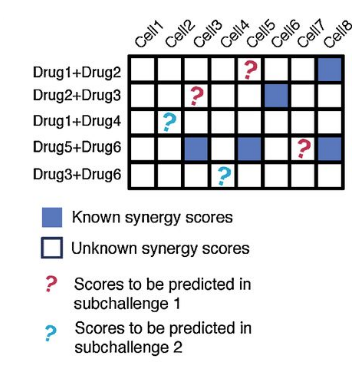
\includegraphics[width=0.4\linewidth]{images/второе соревнование.png}}
\caption{Схематичное представление задач SC1 и SC2 }
\end{figure}


Рассмотрим оценку методов по первому направлению соревнования. Поскольку размер выборки для каждой комбинации препаратов варьируется (например, некоторые комбинации препаратов были протестированы на большем количестве клеточных линий, чем другие), применение корреляции Пирсона непосредственно ко всем показателям синергии потенциально даст больший вес комбинациям лекарств, которые имеют больше экспериментов.
Поэтому для придания равных весов всем комбинациям препаратов в качестве метрики была использована средневзвешенная корреляция Пирсона:
\begin{equation}
    p_w = \frac{\sum_{i=1}^N{\sqrt{n_i-1}*p_i}}{\sum_{i=1}^N {\sqrt{n_i-1}}}
    \label{equation}
\end{equation}
где $n_i$ -число клеточных линий, обработанных данной  комбинацией, N = 167 (число комбинаций, используемых для теста), $p_i$ - коэффициент корреляции Пирсона, рассчитанный для предсказанных и наблюдаемых уровней синергии в пределах одной комбинации препаратов  по возможным клеточным линиям\cite{li2018network}.

Для оценки методов по второму направлению использовали многофакторный дисперсионный анализ (ANOVA).

Команды использовали множество различных подходов к предсказанию синергии лекарств, включая регрессию, деревья решений, случайные леса, Гауссовские процессы, SVM, нейронные сети. Однако производительность методов имела слабую связь с выбранным алгоритмом. Самым лучший метод был  Yuanfang Guan с метриками $p_w_{SC1A}$=0,48, $p_w_{SC1B}=0,45$ и $ANOVA_{SC2}=74.89$ для обеих категорий первого направления соревнования и второго направления, соответственно. Основываясь на метрике для  второго соревнования, метод Y Guan показал значительно лучшие результаты по сравнению с другими командами.

Также для второго направления конкурса был проверен ансамблевый метод, основанный на агрегировании всех представленных моделей. Этим подходом добились скромного улучшения производительности по сравнению с лучшим методом. Это явление называется “мудрость толпы” \cite{kuiper2019community}.


$$\textbf{Метод Yuanfang Guan}$$

Более подробно разберем самую лучшую модель Yuanfang Guan\cite{li2018network}.
Команда разработала три модели:
\begin{itemize}
    \item модель глобальной синергии (GSM) - использует один обучающий набор и делает прогнозы для всех тестовых образцов сразу
    \item модель локальной синергии (LSM) - строит обучающий набор для каждого неизвестного показателя синергии в тестовом наборе данных и делает прогнозы отдельно. Обучающий набор данных LSM представляет собой подмножество пар лекарств в GSM, включая только те пары, когда появляется любой из препаратов в тестируемой паре лекарств.
    \item модель единого лекарственного средства (SDM) - SDM аналогичен LSM, за исключением того, что обучающий набор данных генерируется для каждого препарата, а не для комбинации препаратов
\end{itemize}

Каждая из моделей была разработана с использованием алгоритма случайного леса.

Для второго направления соревнований они использовал ROC-AUC, чтобы оценить эффективность бинарных предсказаний. Обозначили наблюдаемые синергетические оценки > 20 как "1" (наблюдаемая синергия) и оценки < 20 как “0” (наблюдаемая несинергия). Этот порог использовался DREAM. Но, как было упомянуто ранее, для бинарных предсказаний консорциум DREAM использовал многофакторный дисперсионный анализ (ANOVA) для оценки предсказаний.
% \cite{li2018network} A зачем этот тут цитировала?
%Так как это статья от авторов метода Yuanfang Guan, я по ней описываю метод.


$$\textbf{Метод Ranking-system of Anti-Cancer Synergy}$$


Дополнительно рассмотрим модель, которую назвали Ranking-system of Anti-Cancer Synergy (RACS) \cite{sun2015combining}. Эту модель  обучена с частичным привлечением учителя.  То есть используется датасет с малым числом комбинаций, которые известны как синергетические.
Для создания обучающего набора данных использовали 26 синергетических пар противоопухолевых препаратов из базы данных \href{https://drugcomb.fimm.fi/}{Drug Combination Database (DCDB)} в качестве меченых. В исследовании было охвачено 33 протестированных препарата с лекарственными мишенями и транскриптомными профилями конкретных клеточных линий после однократной обработки одиночным препаратом. На основе комбинирования 33 препаратов составили 502 пары немаркированных образцов(во всем обучающем датасете 528 пар).

На основе 13 соединений, предоставленных NCI-DREAM, было составлено 78 попарных комбинаций, которые были использованы в качестве тестового набора данных для клеточной линии β-клеточной лимфомы человека OCI-LY3.

Также был создан еще один набор данных для валидации метода на основе 142 противоопухолевых препаратов, одобренных FDA или проходящих клинические испытания (из баз данных \href{https://go.drugbank.com/?ref=xranks}{DrugBank}, \href{http://db.idrblab.net/ttd/}{Therapeutic Target Database} и \href{https://pubmed.ncbi.nlm.nih.gov/}{PubMed}). 
%Дай, пожалуйста, ссылки на DrugBank, Therapeutic Target Database и PubMed
После удаления соединений без аннотаций gene ontology (GO) или информации о сигнальных путях базы данных \href{https://www.kegg.jp/}{KEGG} осталось 118 препаратов. При их комбинирование было создано 6 877 немеченых пар в качестве тестовых данных для клеточной линии A549 и MCF7.


Изначально было выбрано четырнадцать признаков, охватывающих химическую структуру, фармакологию, функциональные и сетевые свойства лекарственных мишеней, но только семь признаков были идентифицированы как существенно отличающиеся между синергетическими и немечеными парами.


Для предварительного ранжирования был применен полууправляемый метод обучения, включающий многообразный алгоритм ранжирования на основе сходства с меченными парами в пространстве 7 признаков.

Аналогичным образом были протестированы пять параметров, описывающих корреляции между дифференциально экспрессируемыми генами, и два параметра были значительно различны между синергетическими и немечеными образцами. Эти два параметра были использованы в качестве дополнительных транскриптомных  фильтров для улучшения предварительного ранжирования. Первый из них DEG\_Overlap рассчитывается как: 
 \begin{equation}
    DEG\_Overlap = \frac{|A\cap{B}|}{\sqrt{|A|\times|B|}}
    \label{equation}
\end{equation}
 где A и B представляют собой множества дифференциально экспрессированных генов, возмущенные препаратом x и y соответственно.
 
 Второй параметр назывался Pathway\_Coverage и вычислялся по формуле: 
 \begin{equation}
     Pathway\_Coverage = \frac{|(A\cup{B})\cap{N}|}{|N|}
    \label{equation}
\end{equation}
где A и B представляют собой множества дифференциально экспрессированных генов, возмущенные препаратом x и y соответственно, N множество всех генов, связанных с сигнальными путями рака.

Ниже приведена схема метода RACS с предварительным ранжированием и транскриптомными фильтрами.
\begin{figure}[H]
\center{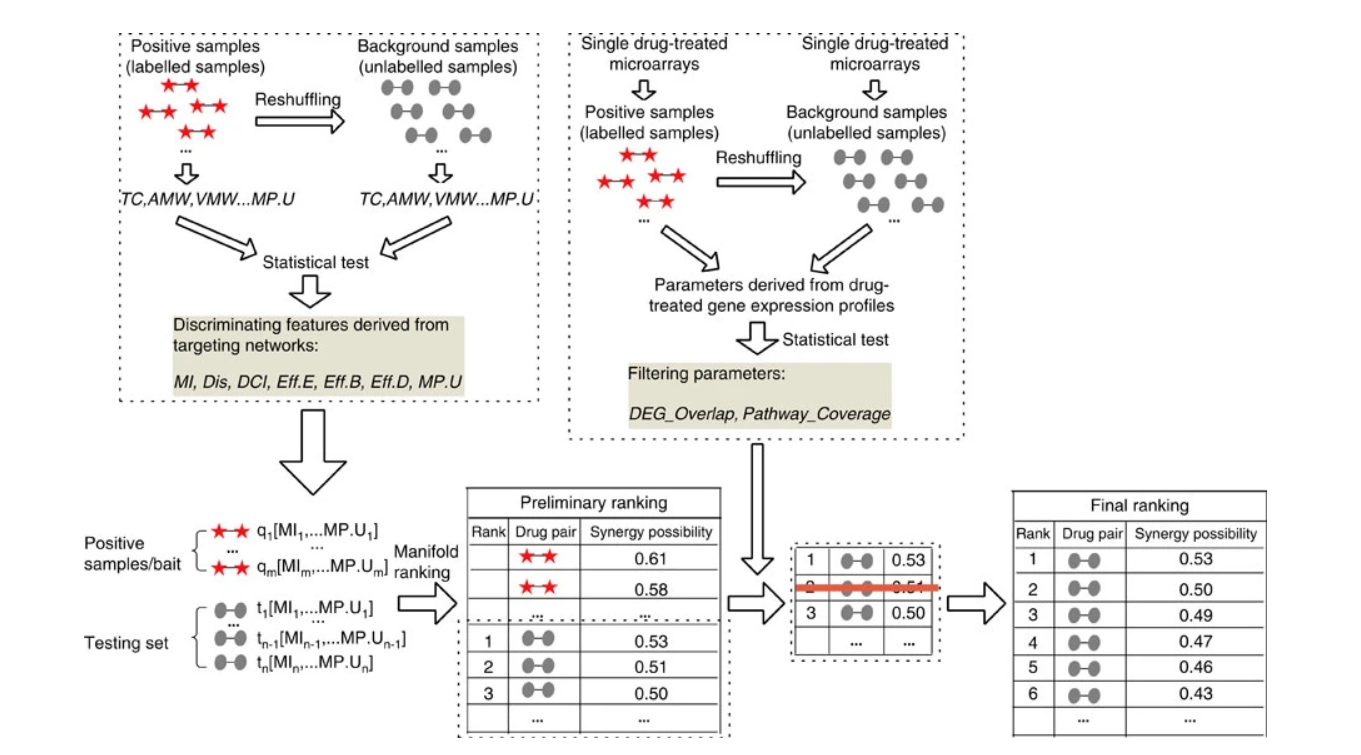
\includegraphics[width=1\linewidth]{images/RACS.png}}
\caption{схема RACS}
\end{figure}



Так как оценка метода была проведена на датасете консорциума DREAM, то метод сравнили с моделями соревнования, о которых было упомянуто выше (среди них выделялись такие методы, как DIGRE, SynGen). В качестве метрик брали ROC-AUC, TPR, PC-index. 



У метод RACS PC-индекс равен 0,78,  ROC-AUC 0,85, то есть этот метод показал наилучшие результаты. 
% Напиши, пожалуйста, как считать ROC-AUC и TPR.
% Выше написала (до разбора отдельных методов)
Именно применение транскриптомных фильтров увеличило PC-индекс с 0,69 до 0,78, а значения ROC-AUC с 0,783 до 0,853.
% Хорошо бы описать что за фильтры
% Я выше описывала, какие признаки использовались для этого. То есть они говорят, что эти признаки значительно отличались у синергетических пар (вероятно были выше):"In this step, we found that for both features of DEG_Overlap and Pathway_Coverage, drug pairs with statistically significant p-values (p<0.05) were enriched in positive samples ." Но как конкретно они фильтруют, я не поняла. Ставят ли они какой-то порог по ним и p-value для этих признаков? Не смогла найти про это подробного описания. 

Также метод был проверен на наборе данных для клеточных линий A549 и MCF7, но с применением других метрик. 

Стоит отметить, что PC-индекс, предложенный консорциум DREAM, более строгий по сравнению с ROC-AUC. PC-index устойчив к возмущениям данных. Например, значение ROC-AUC метода DIGER снизилось с 65 до 48\% после удаления митомицина С из набора из 14 препаратов. Однако PC-индекс метода DIGER оставался почти неизменным. Также он учитывает шум биологических копий. Однако РС-индекс нельзя было использовать для рака молочной железы или легких, потому что вместо биологических копий использовались множественные комбинации различных концентраций.
\newline
\newline

\textbf{Методы с использованием других датасетов}

\newline


$$\textbf{DeepSynergy}$$

Рассмотрим модель DeepSynergy\cite{preuer2018deepsynergy}, которая является методом глубокого обучения. Модель была разработана для задачи регрессии. DeepSynergy была обучена на наборе данных, который включает 23,062 образца, где каждый образец относится к двум соединениям и клеточной линии. Он охватывает 583 различные комбинации, каждая из которых была протестирована против 39 клеточных линий рака, полученных из 7 различных типов тканей. Пары препаратов были построены из 38 противоопухолевых препаратов (14 экспериментальных и 24 одобренных). Среди 38 соединений данные можно поделить на 2 набора:
\begin{itemize}
    \item "исчерпывающий", состоящий из 22 препаратов, у которых все возможные комбинации были протестированы 
    \item "дополнительный", состоящий из 16 препаратов, они были протестированы только в комбинации с препаратами из "исчерпывающего" набора
\end{itemize}
Для каждого образца была измерена скорость роста клеток при обработке комбинацией препаратов в режиме дозирования $4 \times 4$ для 4 биологических копий. Были получены данные монотерапии, то есть зависимость скорости роста клеток при обработке отдельным препаратом для 8 концентраций и 6 биологических копий. На основе этих данных составлялась матрица размером $5\times5$, для которой первая строка и первый столбец являются данными монотерапии. Такие матрицы назывались комбинационнной поверхностью. 

\begin{figure}[H]
\center{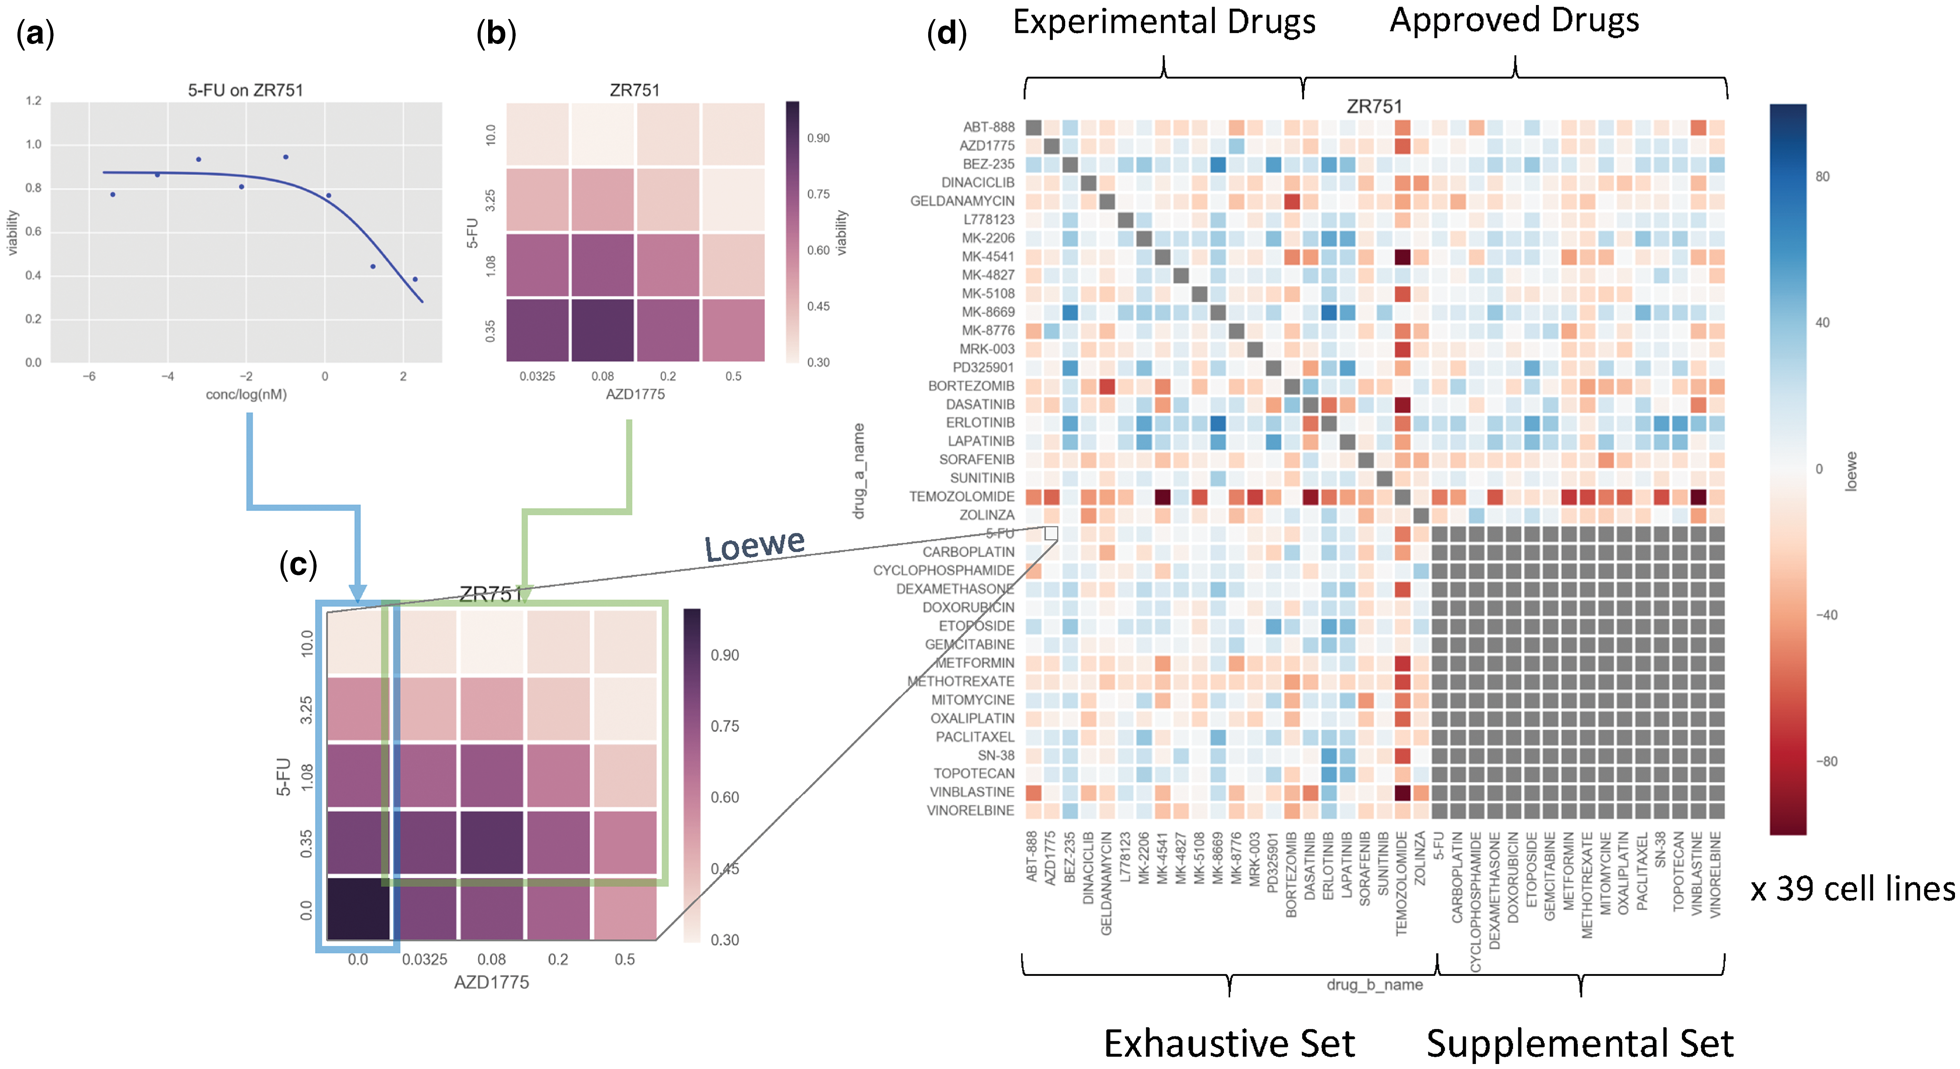
\includegraphics[width=1\linewidth]{images/DDDDDDDDDD.png}}
\caption{Структура датасета}
\end{figure}
Уровень синергии комбинации препаратов вычислялся по комбинационным поверхностям с использованием теоретической модели Loewe Additivity \cite{di2016combenefit}.

Эффект от препаратов A и B с концентрациями a и b соответственно может быть представлен в виде следующей суммы :
\begin{equation}
    E(a,b) = R(a,b) + S(a,b),
\label{equation5}
\end{equation}
где E(a,b) - наблюдаемый в эксперименте эффект, R(a,b) - аддитивный эффект, определяемый по модели Loewe Additivity, S(a,b) - это величина дополнительного эффекта, он положительный в случае синергетического эффекта и отрицательным в случае антагонистического эффекта пары препаратов. 
Аддитивный эффект для комбинации препаратов (a, b) вычисляется путем нахождения двух доз $a_u$ и $b_u$ таких, что:
\begin{equation}
    E(a_u) = E(b_u)
\label{equation}
\end{equation}
Уравнение изоболы (кривой одинакового эффекта):
\begin{equation}
    \frac{a}{a_u}+\frac{b}{b_u} = 1
\label{equation}
\end{equation}
Найдя численное решение этих 2 уравнений, считают аддитивный эффект:
\begin{equation}
    R_{Loewe}(a,b) = E(a_u) = E(b_u)
\label{equation}
\end{equation}
Зная аддитивный и наблюдаемый эффекты, можно посчитать синергетический. Значения синергии варьируются от -326 до 179.
% Опиши, пожалуйста, Loewe Additivity

Использовали как химическую информацию о препаратах, так и геномную информацию, отражающую биологию болезни. Авторы вычислили три различных типа химических признаков: extended connectivity fingerprints с радиусом 6, получены с использованием jCompoundMapper, физико-химические свойства с использованием ChemoPy,  бинарные признаки основанные  на наборе токсикофоров, собранных из литературы. Токсикофоры-это подструктуры, которые токсичны. Пространство химических признаков было уменьшено фильтрацией признаков с нулевой дисперсией. Финальный набор признаков содержал 1309 ECFP\_6, 802 физико-химических и 2276 признаков токсикофоров. Клеточные линии были описаны профилем экспрессии генов. Конечный набор был из 3984 геномных признаков.


Модель DeepSynergy - это нейронная сеть с обратной связью, которая принимает входные векторы, представляющие образцы, и выдает одно значение - уровень синергии. Образцы описываются сцепленными векторами, которые включают в себя признаки двух препаратов и одной клеточной линии. То есть нейроны входного слоя получают значения экспрессии генов клеточной линии и химические дескрипторы обоих препаратов в качестве входных данных. Затем информация распространяется по слоям сети DeepSynergy до тех пор, пока выходной блок не выдаст прогнозируемый показатель синергии. 

Поскольку сеть не должна различать комбинацию лекарств AB, представленную в порядке A-B или B-A, авторы удваивают измерения, представляя каждый образец дважды в обучающем наборе. Один раз свойства препарата используются в порядке А-В и один раз в порядке В-А. Для прогнозирования оба способа представления выборки распространяются по сети и усредняются. Наблюдалось, что DeepSynergy учится предсказывать одно и то же значение для комбинации лекарств AB в порядке A-B и B-A.

Были рассмотрены различные настройки гиперпараметров, а именно разные стратегии нормализации данных, в сочетании с коническими или прямоугольными слоями с различным количеством нейронов. Использовалось два или три скрытых слоя. Кроме того, исследовались различные скорости обучения, а также методы регуляризации. В итоге  DeepSynergy имеет коническую архитектуру с двумя скрытыми слоями, имеющими 8192 нейрона в первом и 4096 во втором скрытом слое. 
 
\begin{figure}[H]
\center{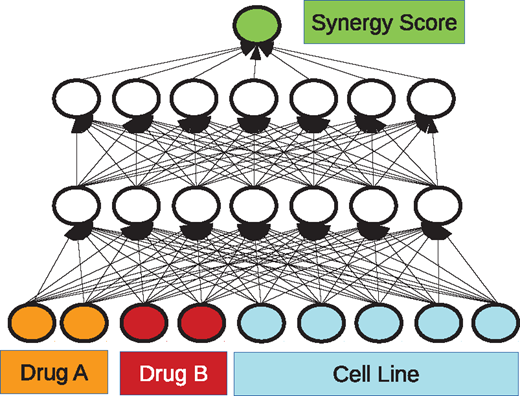
\includegraphics[width=0.4\linewidth]{images/deepsynergy.png}}
\caption{Архитектура DeepSynergy}
\end{figure}
 
В качестве основной метрики оценки модели использовалась среднеквадратичная ошибка (MSE), по которой модель оптимизировалась во время обучения. Также использовали корень из среднеквадратичной ошибки (RMSE) и коэффициент корреляции Пирсона. DeepSynergy достигла тестового MSE: 255, RMSE: 15.91, коэффициент корреляции Пирсона: 0.73. Дополнительно DeepSynergy сравнили со следующими моделями: Median Polish, которая использовалась в качестве базовой случайной модели, Gradient Boosting, Random Forests, Support Vector Machines и Elastic Nets. 
Ниже приведены результаты сравнения на основе вышеперечисленных метрик.
\begin{figure}[H]
\center{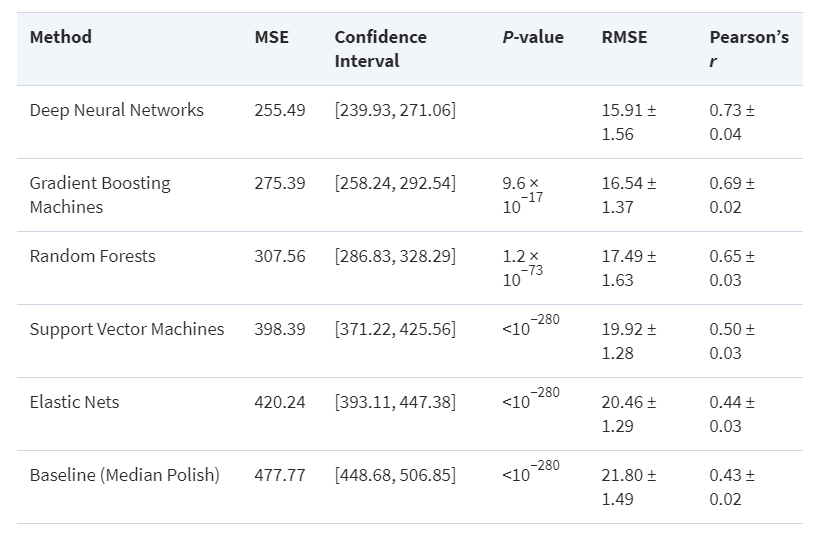
\includegraphics[width=0.7\linewidth]{images/deep_table2.png}}
\caption{Сравнение моделей}
\end{figure}

DeepSynergy показала MSE, равный 255, в то время как Gradient Boosting, Random Forests достигли 275 и 308 соответственно. Support Vector Machines и Elastic Nets показали аналогичные результаты с MSE, равным 398 и 420 соответственно. Median Polish, которая использовалась в качестве базовой, достигла наихудшего результата с MSE 478. Относительное улучшение DeepSynergy по сравнению с базовой моделью составляет 53\%. DeepSynergy значительно превосходит другие методы машинного обучения.



%Добавь, пожалуйста, сюда таблицу 2, плюс дай сравнение с "Median Polish" (сами по себе скоры MSE и RMSE малоинформативны, только в сравнении с рандомом)
Так как RMSE, MSE зависят от набора данных, их трудно использовать для сравнения между различными наборами данных. Поэтому для получения сопоставимых показателей прогностических характеристик DeepSynergy использовались метрики, типичные для задач классификации: ROC AUC, PR AUC, точность (ACC), точность (PREC), чувствительность (TPR), специфичность (TNR). У DeepSynergy  ROC AUC равен 0,9.



$$\textbf{Метод Zhao H.}$$

Для набора данных использовали 184 пары препаратов (на основе 238 препаратов), одобренные FDA orange book. Была собрана молекулярная и фармакологическая информация, связанная с этими препаратами, включая их мишени и соответствующие нисходящие сигнальные пути, области медицинских показаний, терапевтические эффекты, представленные в анатомической терапевтической и химической классификационной системе (АТХ), а также побочные эффекты \cite{zhao2011prediction}.

Для аннотаций лекарственных мишеней использовали данные о взаимодействии соединений и белков из базы данных \href{http://stitch.embl.de/}{STITCH}, \href{https://drugcomb.fimm.fi/}{DrugBank} и базы данных терапевтических мишеней \href{http://db.idrblab.net/ttd/}{TTD}. Далее исследовали пути, на которые возможно воздействует препарат через мишень, информация о сигнальных путях была получена из базы данных \href{https://www.kegg.jp/}{KEGG}. Каждый препарат был связан с путями, в которых состоят его мишени.
% Дай пожалуйста ссылка ни ресурсы
Пара препаратов может быть представлена в виде вектора, состоящего из пар признаков. Например, в случае признака "мишень" препарат 1 связывает два белка {p1, p2}, препарат 2 связывает три белка {p3, p4, p5}, комбинация препарата 1 и препарата 2 может быть представлена в виде следующих пар признаков: {(p1, p3), (p1, p4), (p1, p5), (p2, p3), (p2, p4), (p2, p5)}, аналогично для других признаков.



Затем был проведен поиск тех пар признаков, которые наиболее часто встречаются в синергетических парах. Для пары препаратов ($d_i$, $d_j$) признака F (например, мишень), $f_i$ связан с $d_i$ и $f_j$ с $d_j$ , где $f_i$ и $f_j$ $\subset{F}$ . Пара препаратов ($d_i$, $d_j$) может быть представлена парой признаков ($f_i$, $f_j$). Для каждой пары признаков рассчитывается  оценка обогащения $s_{ij}$ следующим образом:
\begin{equation}
   s_{ij} = \frac{N_{ij}}{N'_{ij}}
    \label{equation}
\end{equation}
где $N_{ij}$ - сколько раз пара признаков встречается в синергетических комбинациях лекарств, $N_{ij}$ - сколько раз  пара признаков встречается в фоновом наборе всех возможных попарных комбинаций между лекарственными средствами, участвующих в синергетических комбинациях лекарств. Таким образом, все пары признаков могут быть ранжированы по $s_{ij}$, то есть по обогащению в синергетических парах.

Затем для выбранного признака F обучали модель предсказывать оценку обогащения для пары признаков комбинации препаратов. Для этого использовали кросс-валидация. В ходе кросс-валидация все комбинации препаратов были случайным образом разделены на пять групп одинакового размера без перекрытия, четыре из которых использовались в качестве обучающего набора и использовались для расчета оценки обогащения для каждой пары признаков, в то время как оставшаяся группа использовалась в качестве валидационного набора, и процедура повторялась в течение пяти раз. Оценка F1 была принята в качестве показателя производительности модели. Порог, выше которого был достигнут самый высокий балл F1 при перекрестной валидации, использовался для предсказания эффективности. То есть пара препаратов считалась синергетической, если оценка обогащения ее пары признаков была выше порогового значения. Таким образом рассмотренная задача относилась к классификации и для сравнение важности признаков использовали метрику ROC-AUC. По ней было отобрано наиболее три важных признака: область терапии, мишень и область показаний. Затем, интегрируя эти признаки, аналогичным образом предсказываем синергетические пары \cite{zhao2011prediction}.

Среди рассмотренных методов наибольшего результата достигли подходы, для которых был доступен обучающий набор данных. Методы, которые могли использовать только молекулярные данные клеточных линий, фармакологические признаки, данные монотерапии и гипотезы механизма синергии, показывали результаты немного выше случайных моделей \cite{bansal2014community}, что говорит о плохом понимании механизмов, лежащих в основе синергии.
 
$$\textbf{L1000CDS$^2$}$$

Рассмотрим еще один метод предсказания синергетических пар малых молекул, используемый в подходе $L1000CDS^2$ \cite{duan2016l1000cds}. В основе работы этого инструмента лежит концепция Connectivity Map \cite{lamb2006connectivity}. Рассмотрим 2 клеточных состояния, например здоровое и больное, либо 2 типа клеток.
%Приведи, пожалуйста, картинку из @article{lamb2006connectivity,
%   title={The Connectivity Map: using gene-expression signatures to connect small molecules, genes, and disease},
%   author={Lamb, Justin and Crawford, Emily D and Peck, David and Modell, Joshua W and Blat, Irene C and Wrobel, Matthew J and Lerner, Jim and Brunet, Jean-Philippe and Subramanian, Aravind and Ross, Kenneth N and others},
%   journal={science},
%   volume={313},
%   number={5795},
%   pages={1929--1935},
%   year={2006},
%   publisher={American Association for the Advancement of Science}
% } чтоб был понятен концепт Connectivity Map
На основе данных RNA-seq для этих 2 состояний можно найти сигнатуру, состоящую из генов с повышенной и пониженной экспрессией. $L1000CDS^2$ производит поиск малых молекул, которые  имитируют или обращают сигнатуру, подданную в качестве входных данных. Этот поиск осуществляется на основе сравнения поданной сигнатуры с сигнатурами клеточных линий, химически возмущенных, из базы данных LINCS-1000. Сигнатуры рассчитываются из данных экспрессии с помощью их собственного метода Characteristic Direction (CD). Для приоритизации малых молекул L1000CDS2 вычисляет косинусное расстояние между вектором входной сигнатуры и сигнатурами в LINCS-L1000.

\begin{figure}[H]
\center{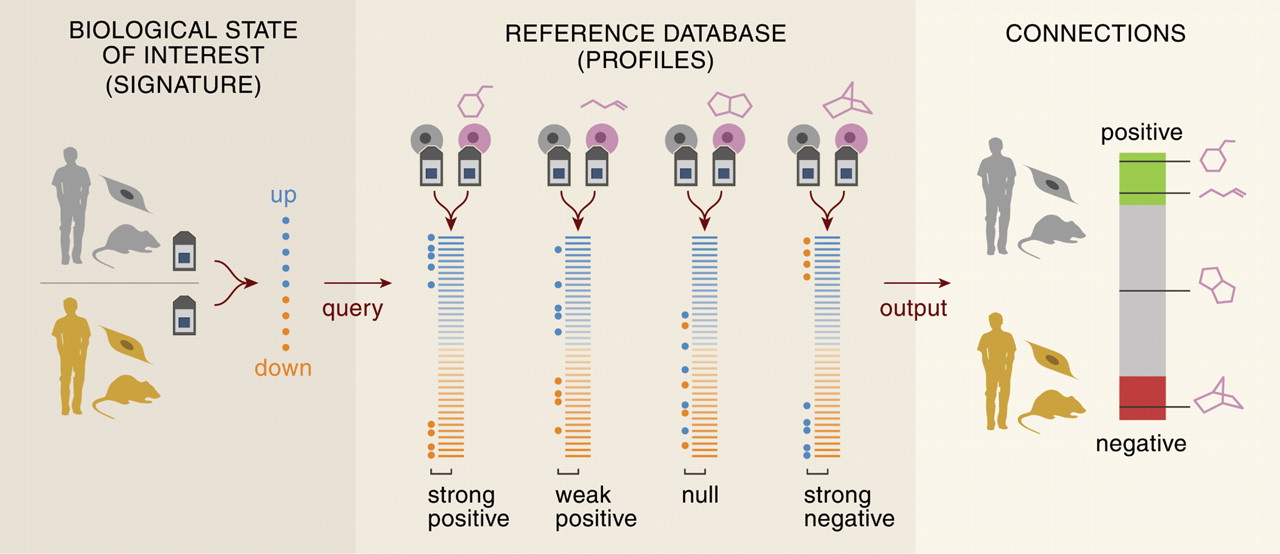
\includegraphics[width=0.7\linewidth]{images/Cmap.jpg}}
\caption{Концепция Connectivity Map\cite{lamb2006connectivity}}
\end{figure}

При поиске синергетических комбинаций L1000CDS2 сравнивает каждую возможную пару из 50 лучших подобранных сигнатур и вычисляет уровень синергии каждой пары, как ортогональность между двумя сигнатурами.
% На вход можно подавать другие сигнатуры запросы кроме output'a CD, поэтому убрала
Идея состоит в том, что если два возмущения ортогональны, то они воздействуют через два независимых пути и вероятно несут комплиментарный синергетический эффект. 

\subsection{Анализ обогащения сигнальных путей}
Повышению доступности технологии секвенирования привело к накоплению большого количества данных. Однако их интерпретация в контексте биологических процессов довольно трудная задача.

Геномное секвенирование показало, что большая часть генов, определяющих основные биологические функции, является общей для всех эукариот. Знания о биологической роли таких общих белков в одном организме часто могут быть перенесены на другие организмы \cite{ashburner2000gene}. Для организации накопленных знаний о функциях групп генов  используются библиотеки наборов генов. Каждая такая библиотека состоит из набора списков связанных генов, где каждый набор генов связан с определенным функциональным термином, таким как название сигнального пути или фактора транскрипции \cite{chen2013enrichr}.

При анализе дифференциальной экспрессии определяются статистически значимые гены с повышенной или пониженной экспрессией (также можно говорить об этих генах в терминах сильной корреляции или антикорреляции с одним из фенотипов). Однако в большинстве случаев представляют интерес затронутые ими биологические процессы. Используя библиотеки наборов генов, можно определить, из каких наборов гены наиболее представлены среди дифференциально экспрессированных генов. Функциональные термины, соответствующие этим наборам генов, говорят о процессах, чья активность претерпела изменения.  

Самый первый метод, который разработал такой подход, назывался анализом обогащения набора генов (GSEA). Принимая список генов, ранжированных по корреляции их профилей экспрессии с одним из двух фенотипов, GSEA стремится оценить значимость избыточного представления независимо определенного набора генов, S, в сильно коррелированных или антикоррелированных генах списка. Для оценки степени обогащения, метод GSEA вычисляет величину значения обогащения, проходя по списку, увеличивая совокупную сумму, когда ген находится в S, и уменьшая ее, если ген не принадлежит списку S. Размер приращения зависит от корреляции генов и фенотипов. Значение обогащения (ES) определяется как максимальное отклонение от нуля совокупной суммы \cite{10.1093/bioinformatics/btm369}.

Было разработано много других инструментов анализа обогащения набора генов с сохранением этой первоначальной концепции. Также стоит упомянуть о самих ресурсах, содержащих ранее упомянутые наборы генов. К самым известным относится \href{http://geneontology.org/}{Gene Ontology}, \href{https://www.kegg.jp/}{KEGG}. 